\documentclass[tikz]{standalone}
\usetikzlibrary{arrows}

\begin{document}

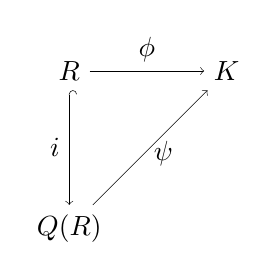
\begin{tikzpicture}
    %%% NODES
    \path (0,0) node(x) {$R$}
    (2,0) node(y) {$K$} (0,-2) node(z) {$Q(R)$};
    %%% LINES
    \draw[very thin,->] (x) --node[above,midway] {$\phi$} (y);
    \draw[very thin,->] (z) --node[right,pos=0.45] {$\psi$} (y);
    \draw[very thin,right hook->] (x) --node[left,midway] {$i$} (z);
\end{tikzpicture}

\end{document}